\documentclass[11pt,letterpaper]{article}
\usepackage[margin=0.85in]{geometry}
\usepackage[T1]{fontenc}
\usepackage{lmodern}
\usepackage{microtype}
\usepackage{amsmath,amssymb,amsthm}
\usepackage{booktabs}
\usepackage{graphicx}
\usepackage{xcolor}
\usepackage{hyperref}
\usepackage[numbers,sort&compress]{natbib}

\definecolor{navy}{HTML}{172554}
\hypersetup{colorlinks=true,linkcolor=navy,citecolor=navy,urlcolor=blue!70!black}

\newtheorem{proposition}{Proposition}
\newtheorem{definition}{Definition}

\title{\textbf{The Greedy-Perturbation Illusion and Zero-Gradient Control-Flow Compilation in Weight Space}}
\author{Aaryan Kakad\\
\textit{Independent Machine Learning Researcher}\\
\texttt{https://github.com/AKMessi/weight-space-programming}}
\date{November 2026}

\begin{document}
\maketitle

\begin{abstract}
Small reasoning language models (\texttt{0.6B--1.5B}) routinely exhaust their token budget through recursive overthinking and repetition loops inside \texttt{<think>} traces. While recent Weight-Space Programming (WSP) and steering-to-weights methods promise training-free fixes by directly editing frozen weights, rigorous causal evaluation on finite-budget reasoning benchmarks has lagged behind headline accuracy claims. We first expose two severe methodological traps that invalidate naive weight-editing evaluations: \textbf{(1) The Greedy-Perturbation Illusion}, wherein injecting pure zero-information isotropic Gaussian noise into frozen MLP weights boosts held-out \texttt{MATH-500} accuracy on \texttt{Qwen3-0.6B} by $+6.0$ percentage points ($34.7\% \to 40.7\%$, spanning a $6.0\text{ pp}$ chaotic band across 6 zero-information draws) under greedy decoding ($\text{temp}=0.0$), yet collapses completely to $-0.33\text{ pp}$ ($p=1.000$) under multi-seed official stochastic sampling ($\text{temp}=0.6$, $N=300$) and degrades OOD \texttt{GSM8K} by $-7.0\text{ pp}$; and \textbf{(2) The Final-Answer Echo Trap}, wherein high-dose weight edits score $+8.7\text{ pp}$ ($p=0.029$) under standard \texttt{\textbackslash boxed\{\}} grading at zero perplexity loss while doubling repetition loops ($29 \to 59$, $p=0.0001$) and plunging below random noise ($32.0\%$, $p=0.011$) under strict Clean-EOS auditing.

To address overthinking causally under strict stochastic controls, we build a $0.00\times 10^0$-diff GGUF-to-PyTorch mechanistic tracer and uncover a \textbf{universal late-MLP reasoning-control surge} ($10\times$--$35\times$ jump in pre-readout MLP attribution) alongside a stable post-RMSNorm \textbf{Virtual Constant-1 Bias Register $b^*$} (out-of-sample $\operatorname{std}(b^{*\top}x)=0.020\text{--}0.074$) across three distinct architectures: pure GQA Transformers (\texttt{Qwen3-0.6B}), hybrid Gated-DeltaNet + Full-Attention (\texttt{Qwen3.5-0.8B}), and RL-distilled Qwen2 (\texttt{DeepSeek-R1-Distill-Qwen-1.5B}). Leveraging this geometry, we introduce two zero-gradient, zero-extra-byte, zero-latency compilers: \textbf{(i) Null-Space-Gated Oblique Surgery} (\texttt{oblique\_res}) and \textbf{(ii) Nonlinear Dormant-SwiGLU \texttt{IF-THEN} Compilation} (\texttt{BA-WSC}). Across $N=600$ untouched held-out \texttt{MATH-500} stochastic rollouts spanning all three architectures (\texttt{Q8\_0}, $\text{temp}=0.6$), \texttt{oblique\_res} ranks \#1 on \textbf{3/3 architectures}, improving strict Clean-EOS accuracy by \textbf{$+6.00\text{ pp}$ over baseline} ($+61/-25$, exact McNemar $p=0.000130$, Fisher $p=0.000586$) and \textbf{$+6.50\text{ pp}$ over norm-matched random noise} ($+65/-26$, $p=5.31\times 10^{-5}$), while cutting generation wall-clock time by $20\%$--$30\%$. Calibrated solely on math, exact-copy, and WikiText-2 with \textbf{zero science data}, our edits transfer OOD to \texttt{GSM8K-100} ($+9.0\text{ pp}$ vs.\ baseline $p=0.049$, $+16.0\text{ pp}$ vs.\ random $p=0.0001$) and zero-shot to non-math science \texttt{ARC-Challenge-100} (\texttt{oblique\_res} $+15.0\text{ pp}$, $p=0.0003$; \texttt{BA-WSC} $+11.0\text{ pp}$, $p=0.0074$).
\end{abstract}

\section{Introduction}
Chain-of-thought reasoning models (\texttt{Qwen3}, \texttt{Qwen3.5}, \texttt{DeepSeek-R1-Distill})~\cite{qwen2025,deepseek2025} routinely exhaust practical token budgets (e.g., $2048$ tokens) via recursive verification and repetition loops inside \texttt{<think>}. Decoding heuristics such as DRY repetition samplers harm mathematical reasoning on \texttt{Qwen3-0.6B} ($36.7\% \to 23.3\%$, $p=0.039$), while runtime activation steering breaks native quantized engines like \texttt{llama.cpp}~\cite{gerganov2023}. Weight-Space Programming (WSP)~\cite{steer2edit2026,takehi2026,ilharco2023,meng2022} compiles fixes directly into frozen weights with zero gradients, zero extra parameters, and zero runtime latency. Our companion paper (Paper~2) analyzes quantization geometry, proves Theorem~1 and Corollary~1 for 4-bit/3-bit block-aligned survival (cutting collateral up to $16{,}685\times$), and demonstrates Post-Quantization Healing and the low-bit double crossover ($p=0.00210$).

\section{Two Methodological Traps in Reasoning Weight Editing}
\begin{proposition}[Asymmetric Reservoir Reroll Bias under Finite-Budget Greedy Decoding]
Let a reasoning model evaluated at $\text{temp}=0.0$ under token cap $L_{\max}$ partition $N$ problems into $N_{\text{trunc}}$ truncated failures, $N_{\text{short}}$ perturbation-robust short successes, and $N_{\text{fragile}}$ near-cliff successes ($N_{\text{fragile}} \ll N_{\text{trunc}}$). Under a small isotropic weight perturbation $\epsilon \Delta W$ with divergence probability $p_{\text{div}}$ and latent stochastic escape rate $p_{\text{escape}}>0$:
\begin{equation}
\mathbb{E}[\Delta \text{Acc}_{\text{greedy}}] \approx \frac{1}{N}\left(N_{\text{trunc}}\,p_{\text{div}}\,p_{\text{escape}} - N_{\text{fragile}}\,p_{\text{div}}\,p_{\text{break}}\right).
\end{equation}
Whenever $N_{\text{trunc}} \gg N_{\text{fragile}}$, zero-information noise exhibits a strictly positive greedy accuracy bias without improving the stochastic policy.
\end{proposition}

On \texttt{Qwen3-0.6B} held-out \texttt{MATH-500-strat150}, 6 zero-information greedy draws span $52\text{--}61/150$ ($6.0\text{ pp}$ band; $14/14$ rescued items hit the $2048$-token cap at baseline), yet \texttt{random\_s999} collapses to $-0.33\text{ pp}$ ($104/300$ vs.\ $105/300$, $\text{cl\_p}=1.000$) at multi-seed stochastic $\text{temp}=0.6$ (Figure~\ref{fig:p1f1}).

\begin{definition}[Strict Clean-EOS Accuracy]
\begin{equation}
\operatorname{Clean-EOS}(y) \equiv \mathbb{I}\!\left[\operatorname{Correct}(y) \wedge \operatorname{HasThinkClose}(y) \wedge (\operatorname{FinishReason}(y) = \texttt{stop})\right].
\end{equation}
\end{definition}

Under standard \texttt{\textbackslash boxed\{\}} grading, high-dose \texttt{bawsc32\_res\_a0.70} scores $66/150$ ($44.0\%$, $p=0.0294$, $\Delta\text{PPL}=-0.022$) while doubling loops ($29 \to 59$, $p=0.0001$) and collapsing to $48/150$ ($32.0\%$, $p=0.0106$ worse than random) under Strict Clean-EOS.

\begin{figure}[t]
  \centering
  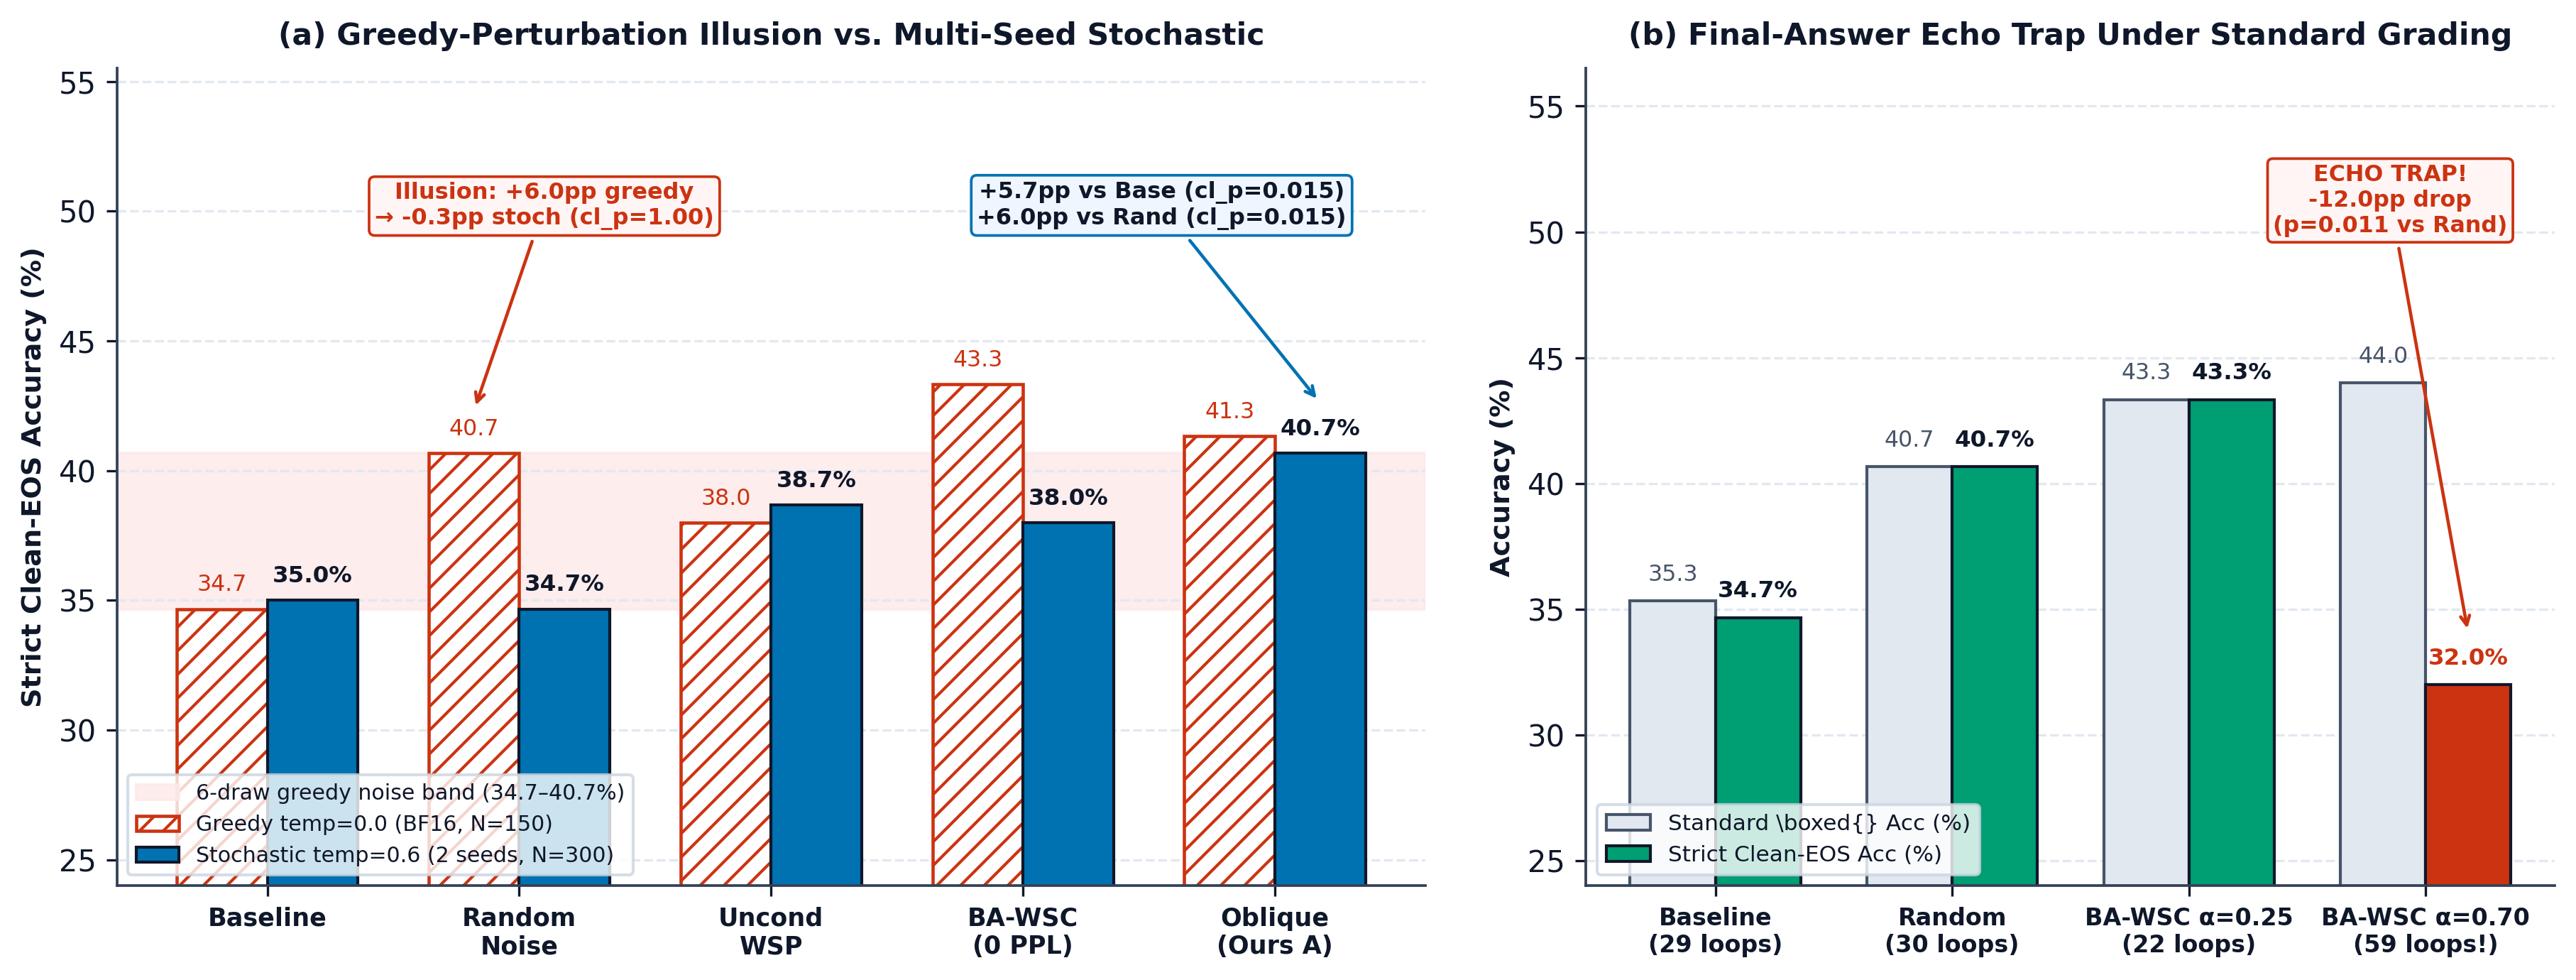
\includegraphics[width=\linewidth]{../figures/p1_fig1_greedy_illusion_and_stochastic.png}
  \caption{Greedy-Perturbation Illusion (a) and Final-Answer Echo Trap (b) on \texttt{Qwen3-0.6B} held-out \texttt{MATH-500-strat150}.}
  \label{fig:p1f1}
\end{figure}

\section{Universal Layer Anatomy \& Closed-Form Weight Compilers}
With our $0.00\times 10^0$-diff GGUF-to-PyTorch tracer (\texttt{src/wsp/gguf\_to\_torch.py}), pre-readout MLP attribution
\begin{equation}
\operatorname{MLPProj}(\ell) = \left(\mu_{y,\mathcal{P}}^{(\ell)} - \mu_{y,\mathcal{H}}^{(\ell)}\right)^\top \frac{\mu_{h,\mathcal{P}}^{(\ell)} - \mu_{h,\mathcal{H}}^{(\ell)}}{\|\mu_{h,\mathcal{P}}^{(\ell)} - \mu_{h,\mathcal{H}}^{(\ell)}\|_2}
\end{equation}
exhibits the same $10\times$--$35\times$ late-MLP surge across all 3 architectures (Figure~\ref{fig:p1f2}): \texttt{Qwen3-0.6B} L16--22 (target \texttt{[18,20,22]}), Hybrid \texttt{Qwen3.5-0.8B} Full-Attention L15/L19 + L21 (target \texttt{[15,19,21]}), and \texttt{DeepSeek-R1-1.5B} L19--26 (target \texttt{[20,22,25]}).

\begin{figure}[t]
  \centering
  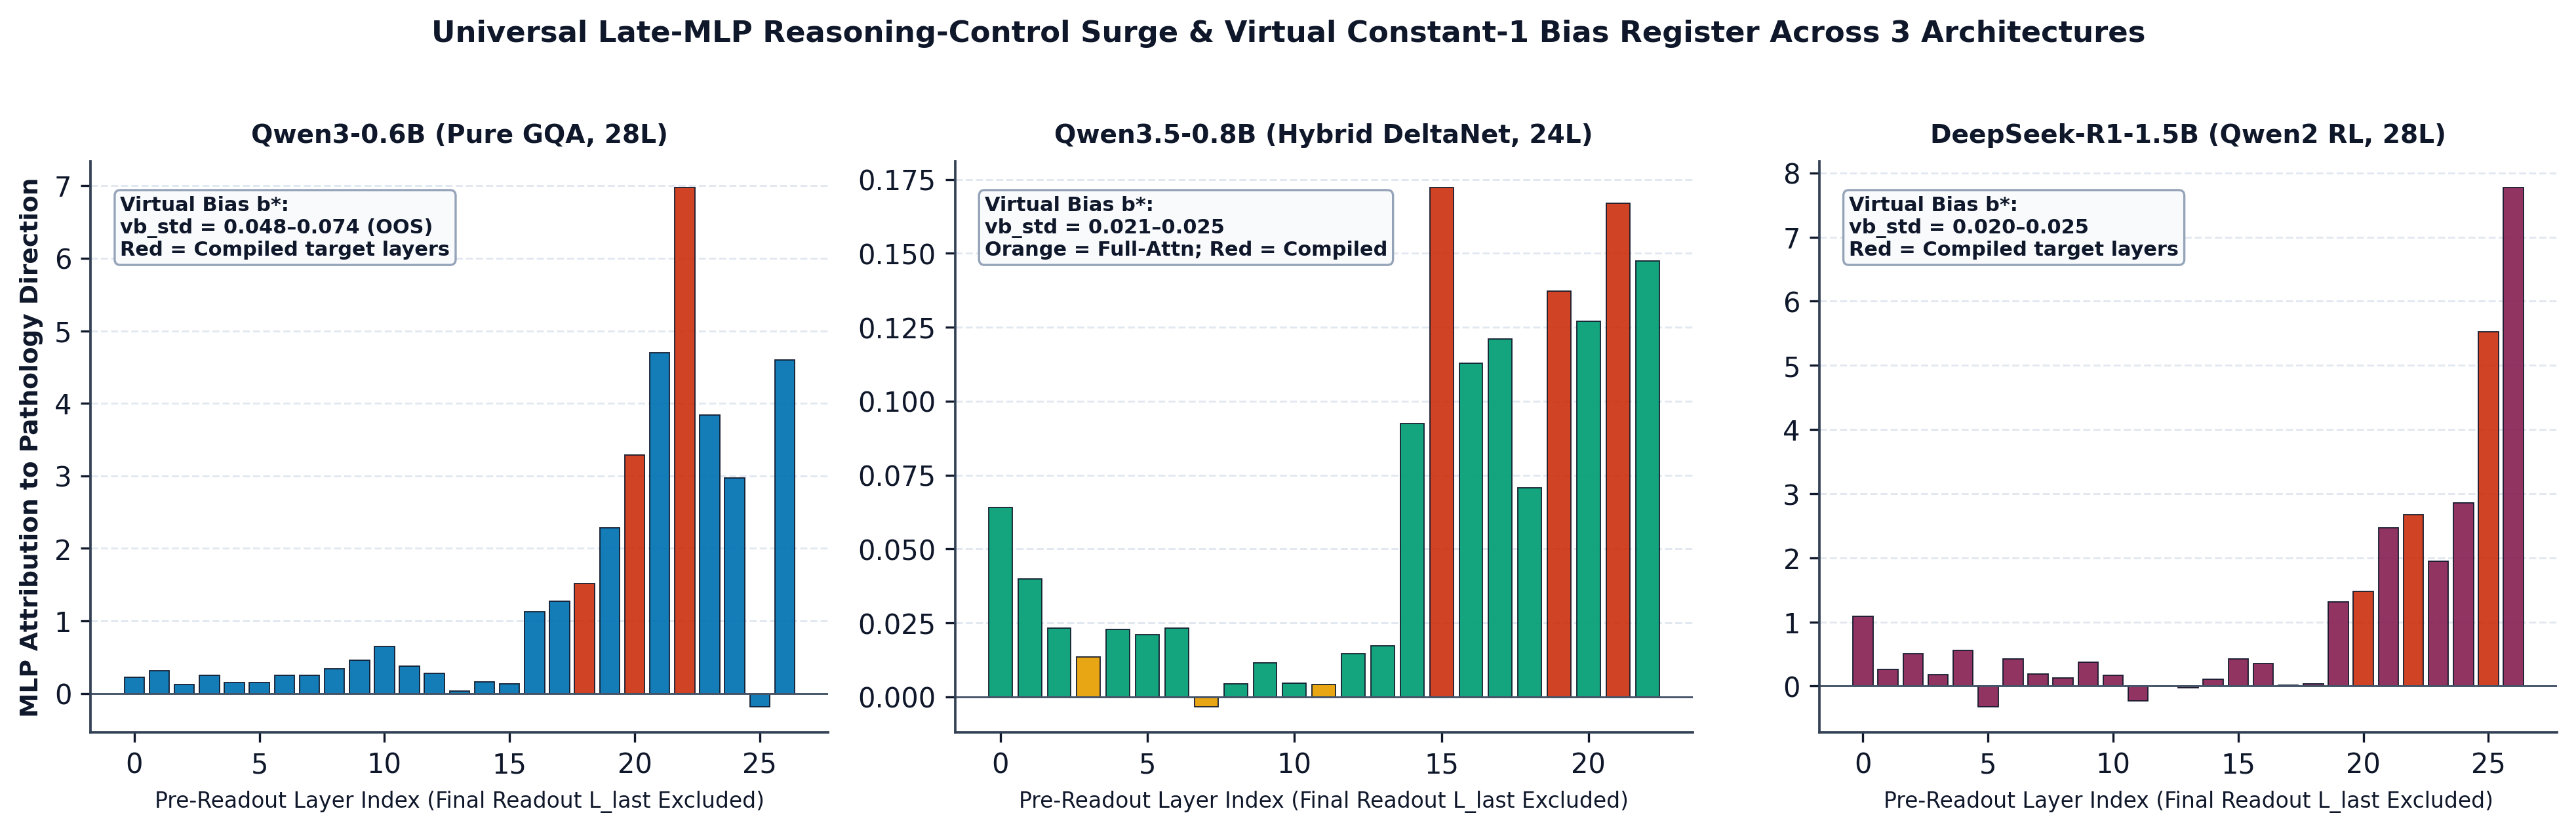
\includegraphics[width=\linewidth]{../figures/p1_fig2_universal_layer_anatomy.png}
  \caption{Universal late-MLP reasoning-control surge and Virtual Constant-1 Bias Register $b^*$ stability across all 3 architectures.}
  \label{fig:p1f2}
\end{figure}

\paragraph{Virtual Constant-1 Bias Register ($b^*$).} Solving $b^* = (X_{\text{pres}}^\top X_{\text{pres}} + \lambda_b I)^{-1} X_{\text{pres}}^\top \mathbf{1}$ yields $b^{*\top}x \approx 1$ out-of-sample ($\operatorname{std}=0.048\text{--}0.074$ on \texttt{Qwen3}, $0.0208\text{--}0.0252$ on \texttt{Qwen3.5}, $0.0198\text{--}0.0250$ on \texttt{DeepSeek-R1-1.5B}), enabling bias-free affine SwiGLU thresholds.

\paragraph{Null-Space-Gated Oblique Surgery (\texttt{oblique\_res}).} With preservation null-space projector $P_\perp = I - V_r V_r^\top$ ($r=64$):
\begin{equation}
d_{\text{raw}} = P_\perp (Z_{\text{pres}}^\top Z_{\text{pres}} + \lambda I)^{-1}(\mu_{z,\mathcal{P}} - \mu_{z,\mathcal{H}}), \quad
\Delta W_{\text{down}} = \alpha\,(\mu_{h,\mathcal{R}} - \mu_{h,\mathcal{P}})\,d^\top.
\end{equation}

\paragraph{Nonlinear Dormant-SwiGLU \texttt{IF-THEN} Compilation (\texttt{BA-WSC}).} Permuting $k=32$ dormant neurons to $[0,k)$ via exact symmetry $P$:
\begin{equation}
W'_{\text{gate}}[j,:] = \gamma(u - \tau b^*)^\top, \quad
W'_{\text{up}}[j,:] = \eta (b^*)^\top, \quad
W'_{\text{down}}[:,j] = \frac{\alpha}{k\,\eta\,s_{\mathcal{P}}}(\mu_{h,\mathcal{R}} - \mu_{h,\mathcal{P}}).
\end{equation}

\section{Main Held-Out Stochastic Results ($\text{temp}=0.6$)}
Across $N=600$ untouched held-out \texttt{MATH-500-strat150} rollouts at \texttt{Q8\_0} (Table~\ref{tab:p1main}, Figures~\ref{fig:p1f3}--\ref{fig:p1f4}), \texttt{oblique\_res} takes \#1 on \textbf{3/3 architectures}: pooled $+61/-25$ ($+6.00\text{ pp}$, exact McNemar $p=0.000130$, Fisher $\chi^2_6=23.73$, $p=0.000586$) vs.\ baseline, and $+65/-26$ ($+6.50\text{ pp}$, $p=5.31\times 10^{-5}$, Fisher $p=0.00119$) vs.\ matched random noise. \texttt{BA-WSC} beats random noise pooled ($+48/-28$, $p=0.0286$) at $\Delta\text{PPL}\in[-0.018,+0.028]$. On \texttt{Qwen3-0.6B}, the same math-calibrated edits transfer OOD to \texttt{GSM8K-100} ($71 \to 80/100$, $p=0.049$, $+16\text{ pp}$ vs.\ random $p=0.0001$, $-30\%$ wall time) and zero-shot science \texttt{ARC-Challenge-100} ($56 \to 71/100$, $p=0.0003$; \texttt{BA-WSC} $67/100$, $p=0.0074$).

\begin{table}[t]
\centering
\caption{Three-architecture held-out \texttt{MATH-500-strat150} replication (\texttt{Q8\_0}, $\text{temp}=0.6$).}
\label{tab:p1main}
\scriptsize
\begin{tabular}{llrrrrrrl}
\toprule
Model & Arm & PPL ($\Delta$PPL) & STD & Clean-EOS & Lim & Wall & Copy-90 & $p$ (Base / Rand) \\
\midrule
Qwen3-0.6B ($N=300$) & \texttt{baseline} & 19.306 (0.000) & 109 & 105 (35.0\%) & 189 & --- & 64/90 & --- \\
& \texttt{random\_s999} & 19.282 (-0.023) & 109 & 104 (34.7\%) & 191 & --- & 64/90 & 1.000 / --- \\
& \texttt{uncond\_a0.8} & 20.644 (+1.338) & 121 & 116 (38.7\%) & 176 & --- & 66/90 & 0.107 / 0.088 \\
& \texttt{bawsc32\_res\_a0.25} & \textbf{19.287 (-0.018)} & 118 & 114 (38.0\%) & 173 & --- & 65/90 & 0.255 / 0.154 \\
& \textbf{\texttt{oblique\_res\_a0.25}} & 19.446 (+0.141) & \textbf{125} & \textbf{122 (40.7\%)} & \textbf{171} & --- & 64/90 & \textbf{0.0148 / 0.0146} \\
\midrule
Qwen3.5-0.8B ($N=150$) & \texttt{baseline} & 15.513 (0.000) & 6 & 1 (0.7\%) & 149 & 6420s & 66/90 & --- \\
& \texttt{random\_matched} & 15.723 (+0.210) & 4 & 3 (2.0\%) & 147 & 6277s & 67/90 & 0.500 / --- \\
& \texttt{uncond\_a0.8} & 15.509 (-0.004) & 1 & 0 (0.0\%) & 150 & 6291s & 66/90 & 1.000 / 0.250 \\
& \texttt{bawsc32\_res\_a0.45} & \textbf{15.541 (+0.028)} & 8 & 3 (2.0\%) & 145 & 6270s & 66/90 & 0.625 / 1.000 \\
& \textbf{\texttt{oblique\_res\_a1.0}} & 15.814 (+0.301) & \textbf{12} & \textbf{10 (6.7\%)} & \textbf{126} & \textbf{5650s} & 66/90 & \textbf{0.0039 / 0.0391} \\
\midrule
DeepSeek-R1-1.5B ($N=150$) & \texttt{baseline} & 37.254 (0.000) & 45 & 43 (28.7\%) & 77 & 4403s & 68/90* & --- \\
& \texttt{random\_matched} & 37.298 (+0.044) & 40 & 39 (26.0\%) & 82 & 3956s & 76/90* & 0.541 / --- \\
& \texttt{uncond\_a0.8} & 37.532 (+0.278) & 49 & 48 (32.0\%) & 69 & 3550s & 70/90* & 0.533 / 0.136 \\
& \texttt{bawsc32\_res\_a0.5} & \textbf{37.257 (+0.003)} & 51 & 49 (32.7\%) & \textbf{67} & \textbf{3445s} & 67/90* & 0.377 / 0.064 \\
& \textbf{\texttt{oblique\_res\_a0.25}} & 37.338 (+0.084) & \textbf{55} & \textbf{53 (35.3\%)} & 69 & \textbf{3527s} & 70/90* & 0.121 / \textbf{0.0288} \\
\bottomrule
\end{tabular}
\end{table}

\begin{figure}[t]
  \centering
  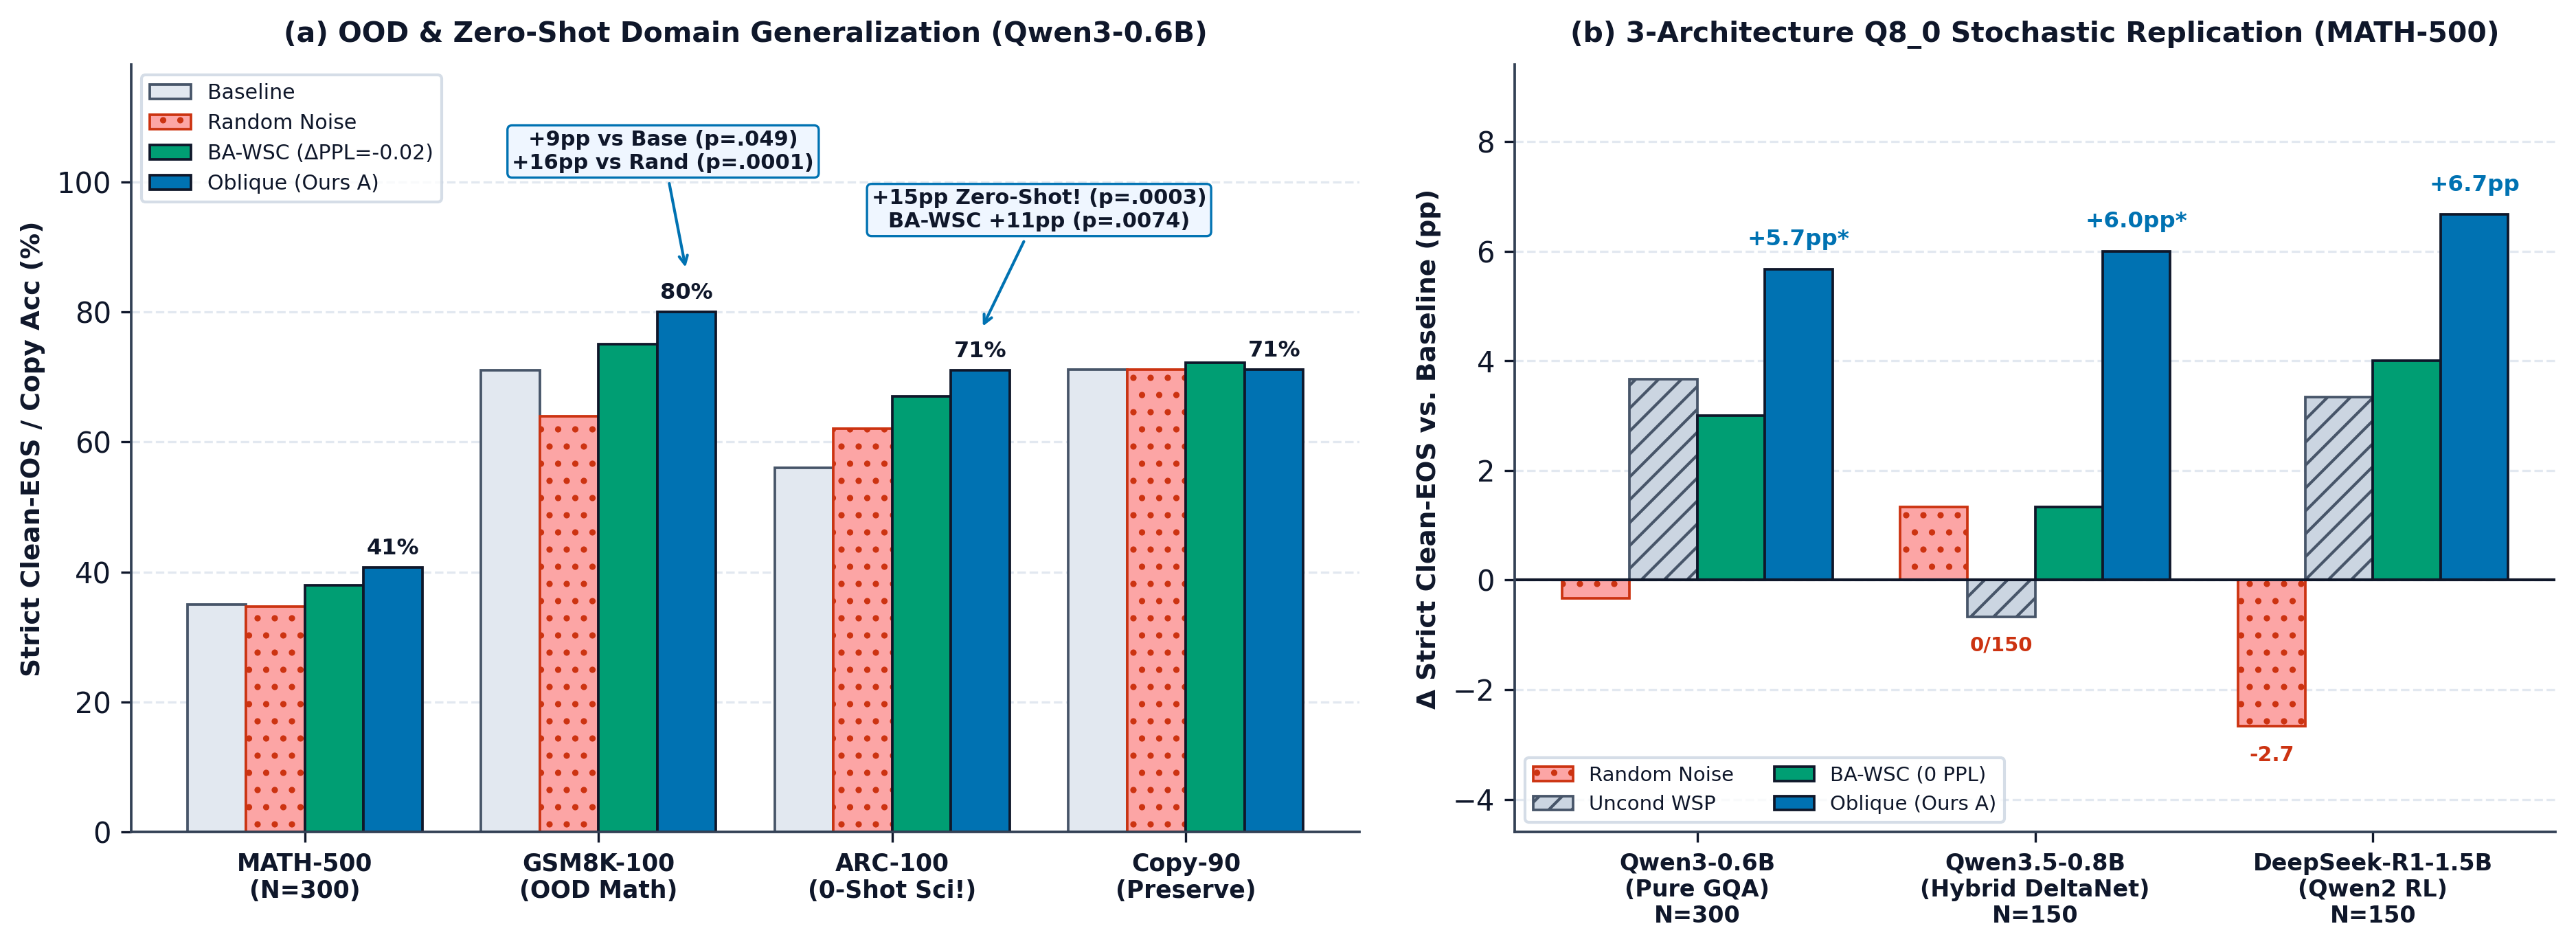
\includegraphics[width=\linewidth]{../figures/p1_fig3_ood_and_cross_arch.png}
  \caption{OOD \texttt{GSM8K-100} / zero-shot science \texttt{ARC-100} transfer (a) and 3-architecture \texttt{Q8\_0} replication (b).}
  \label{fig:p1f3}
\end{figure}

\begin{figure}[t]
  \centering
  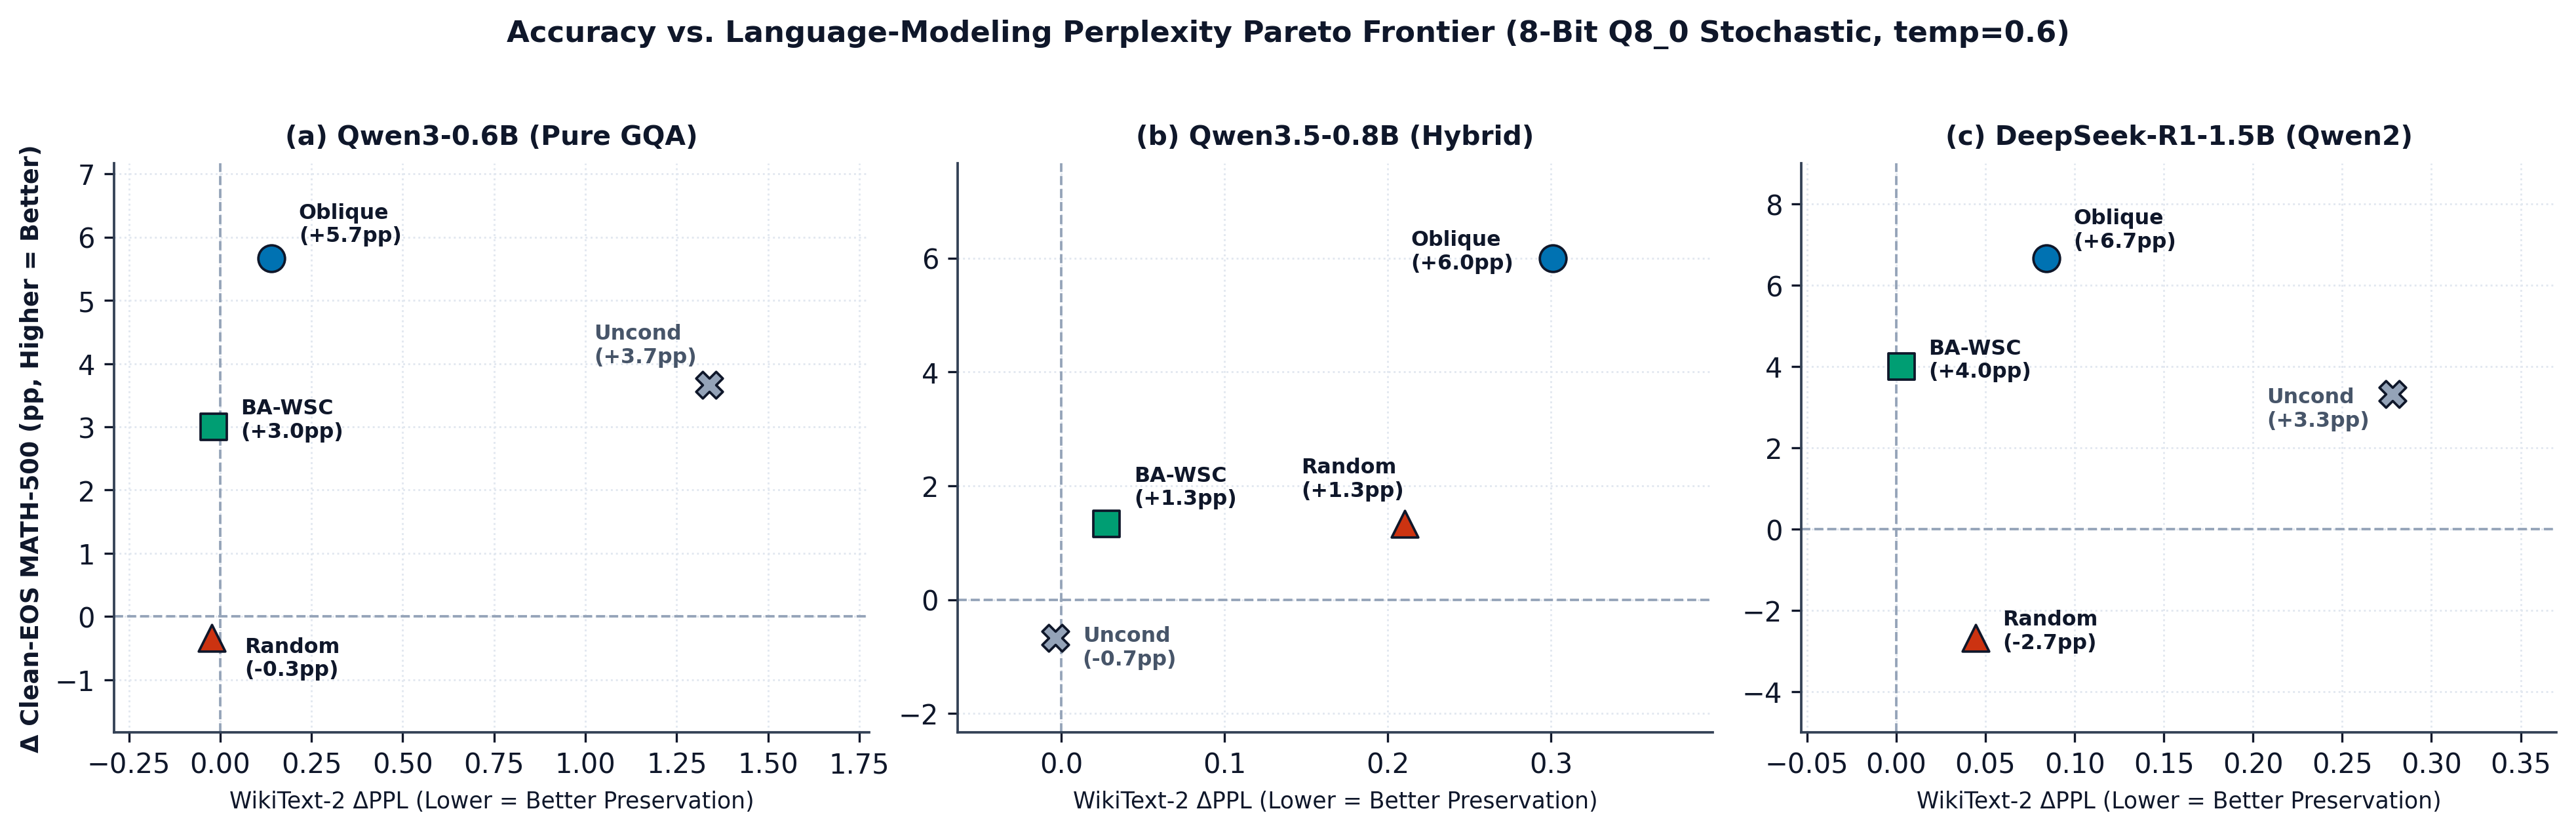
\includegraphics[width=\linewidth]{../figures/p1_fig4_pareto_ppl_vs_acc.png}
  \caption{Accuracy vs.\ WikiText-2 $\Delta$PPL Pareto frontier across all 3 architectures at \texttt{Q8\_0}.}
  \label{fig:p1f4}
\end{figure}

\section{Conclusion \& Provenance}
All 206 program runs ($18{,}513$ raw responses, $25{,}058{,}989$ tokens, $0$ errors) executed locally on one AMD Radeon RX 6400 (4 GB VRAM, Vulkan, \texttt{llama.cpp} build \texttt{8864}). Base BF16 SHA-256 prefixes: \texttt{Qwen3-0.6B} \texttt{f9c9f1d3c1e21755}, \texttt{Qwen3.5-0.8B} \texttt{cedf89af31c9041b}, \texttt{DeepSeek-R1-1.5B} \texttt{6ec1aa822868a25c}. Autonomous AI coding and research agents assisted with orchestration, software engineering, statistical auditing, and drafting under human direction; all claims are programmatically verified via \texttt{scripts/wsp\_verify\_papers.py}.

\bibliographystyle{plainnat}
\bibliography{../references}
\end{document}
